\documentclass[a4paper, fontsize=11pt]{beamer}
\usetheme{Berlin}
\usepackage{mathtools}
\usepackage{fontspec}
\defaultfontfeatures{Ligatures=TeX, Scale=MatchLowercase}
\newcommand{\euro}{€}
\usepackage{polyglossia}
\setdefaultlanguage[spelling=new]{german}
\setotherlanguage[variant=british]{english}
\usepackage[backend=biber, alldates=iso, style=iso-authoryear]{biblatex}
\usepackage[section]{placeins}
\usepackage[newfloat=true]{minted}
\SetupFloatingEnvironment{listing}{name=Quellcode}
\SetupFloatingEnvironment{listing}{listname=Quellcodeverzeichnis}
\usepackage{csquotes}
\usepackage{longtable, booktabs}
\usepackage{graphicx, grffile}
\usepackage{hyperref}
\usepackage[acronym, toc]{glossaries}
\setlength{\parskip}{\medskipamount}
\begin{document}
\begin{frame}
    \author{Mirko Lelansky}
    \title{Kolloquium: Evaluation aktueller Bibliotheken für Stream Graph Processing}
    \date{29.03.2019}
    \maketitle
\end{frame}

\begin{frame}
    \tableofcontents
\end{frame}

\section{Einführung}
\begin{frame}{Hintergründe}
    \begin{itemize}
        \item stetige Datenerzeugung
        \item Verarbeitung der Daten um Mehrwert zu generieren
        \item zum Beispiel welche Produkte liegen aktuell im Trend
        \item schnelle Ergebnisse gefordert
        \item durch Fortschritt und Entwicklung riesiger Datensprung
        \item unterschiedlich strukturierte Daten
    \end{itemize}
\end{frame}

\begin{frame}{Graphen}
    \begin{itemize}
        \item komplexe Datenstruktur $ G = (V,E)$
        \item Liste von Knoten und Liste von Kanten
        \item Kante ist ein un- bzw. geordnetes Paar von Kanten
        \item Weg ist eine Menge von zusammenhängen Kanten
        \item spezielle Klassen von Wegen stellen Spezialfälle dar
    \end{itemize}
\end{frame}

\begin{frame}{Problemstellung}
    \begin{itemize}
        \item unterschiedliche Anforderungen
        \item große Datenmengen
        \item schnelle Antwortzeiten
        \item komplexe Datenstrukturen
        \item Darstellung von Graphen für Verarbeitung
    \end{itemize}
\end{frame}

\begin{frame}{Aufgabenstellung}
    \begin{itemize}
        \item Bibliotheken suchen und wählen
        \item Bibliotheken anhand ihrere Eigenschaften vergleichen
        \item Funktionen demonstrieren
        \item mögliche Einstiegspunkte bzw. Erweiterungspunkte herausarbeiten
    \end{itemize}
\end{frame}

\begin{frame}{Motivation}
    \begin{itemize}
        \item tiefer in die Streaming-Materie einsteigen
        \item Verständnis von Graphen erweitern
        \item alternative BigData-Anwendung kennenlernen
    \end{itemize}
\end{frame}

\section{Theorie}
\begin{frame}{BigData-Methoden}
    \begin{itemize}
        \item zwei große BigData-Methoden
        \item Batch-Processing und Stream-Processing
        \item Batch-Processing arbeitet auf einem großen Datenblock
        \item Stream-Processing arbeitet auf einem kontinuierlichen Datenstrom
    \end{itemize}
\end{frame}

\begin{frame}{Entwicklung von Streaming}
    \begin{itemize}
        \item Streaming ist keine neue Idee, sondern wurde bereits als Modell
            1980 entwickelt
        \item RAM-Maschine verarbeitet einen Stream, eine Folge von Zeichen aus
            einem Alphabet
        \item Parameter der RAM-Maschine sind die Speichergröße und die Anzahl
            der Durchläufe
        \item spätere Modelle machen Einschränkungen auf der Speichergröße
            oder den Durchläufen, bzw. erlauben zusätzliche Methoden auf dem
            Stream
    \end{itemize}
\end{frame}

\begin{frame}{Vorstellung der Bibliotheken}
    \begin{itemize}
        \item gelly-streaming(KTH Schweden), graphstream-project(LITIS),
            Gephi(Universität of Technologie of Compiègne)
        \item gelly-streaming ist eine Bibliothek für Apache Flink, die anderen
            Bibiliotheken sind eigenständig
        \item verschiedene Ansätze, welche alle noch teilweise im experimentellen
            Stadium sind
        \item gelly-streaming(Apache Flink), graphstream-project(Anwendung),
            Gephi(Client-Server)
    \end{itemize}
\end{frame}

\begin{frame}{Vergleich der Bibliotheken}
    \begin{table}
        \begin{tabular}{l|c|c|c}
            Kriterium & gelly-streaming & graphstream-project & Gephi \\
            \hline
            Generatoren & (o) & + & + \\
            Algorithmen & o & o & - \\
            Verteilung & + & - & - \\
            Connectoren & + & o & o \\
        \end{tabular}
    \end{table}
\end{frame}

\section{Analyse und Umsetzung}
\begin{frame}{Beschreibung des Beispieles}
    \begin{itemize}
        \item Ziel: Bipartiteheit eines Graphen
        \item Alternative: Zwei-Farbenproblem eines Graphen
        \item mehrere mögliche Algorithmen
        \item nur für kleine Graphen per Hand lösbar
    \end{itemize}
\end{frame}

\begin{frame}{Beispiel Graph}
    \centering
    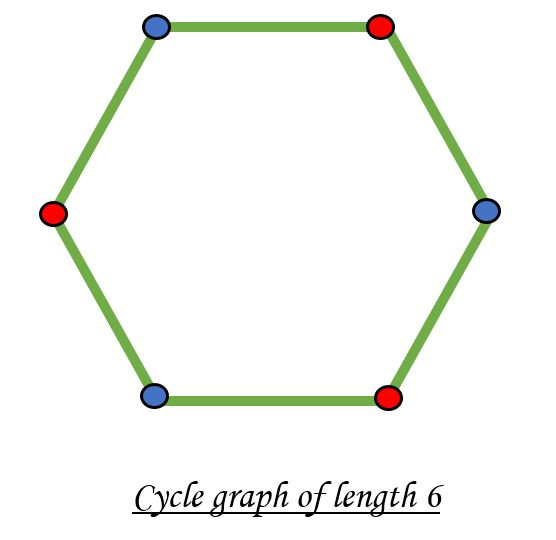
\includegraphics[scale=0.5]{../material/images/bipartite-graph-six-nodes.jpg}
\end{frame}

\begin{frame}{Ablauf des Beispiel (EVA)}
    \begin{itemize}
        \item Einlesen der Daten
            \begin{itemize}
                \item gelly-streaming hat Freiheitsgrade
                \item die anderen Bibliotheken haben Protokoll
            \end{itemize}
        \item Verarbeitung der Daten
            \begin{itemize}
                \item gelly-streaming nutzt Infrastruktur von Apache Flink
                \item graphstream-project nutzt normale Java-Techniken
                \item Gephi nutzt Event-Listener
            \end{itemize}
        \item Ausgabe der Daten
            \begin{itemize}
                \item gelly-streaming Ausgabe erfolgt über Apache Flink
                \item graphstream-project Ausgabe individuell
                \item Gephi Ausgabe über UI
            \end{itemize}
    \end{itemize}
\end{frame}

\begin{frame}{Umsetzung}
    \begin{itemize}
        \item verschiedene Design für die Bibliotheken erstellt
        \item Umsetzung in gelly-streaming erfolgreich (\textbf{Apache Flink 1.2.0!})
        \item Umsetzung in graphstream-project erfolgreich
        \item Umsetzung in Gephi nicht erfolgreich
    \end{itemize}
\end{frame}

\begin{frame}{offene Punkte}
    \begin{itemize}
        \item allgemein
            \begin{itemize}
                \item unterschiedliche Darstellungen
                \item verhalten bei großen Datenmengen
                \item Integration der Bibliotheken mit Neo4J
            \end{itemize}
        \item speziell
            \begin{description}
                \item[gelly-streaming] Speicherung des Graphen
                \item[graphstream-project] Unterbau im Verhältnis zu Apache Flink
                    speziell für Verteilung
                \item[Gephi] apassen der Infrastruktur
            \end{description}
    \end{itemize}
\end{frame}

\section{Zusammenfassung}
\begin{frame}{Fazit}
    \begin{itemize}
        \item Bibliotheken wurden allgemein verglichen
        \item verschieden Designs wurden für die jeweiligen Bibliotheken erzeugt
        \item nicht alle Designs konnten umgesetzt werden
        \item die Bibliotheken haben verschiedene Ansätze
        \item alle habe noch experimentellen Status -> nicht für produktiven
            Einsatz geeignet
    \end{itemize}
\end{frame}

\begin{frame}{Quellen}
    \begin{itemize}
        \item Masterarbeit
    \end{itemize}
\end{frame}
\end{document}
